\documentclass[tikz,border=2pt]{standalone}
\usepackage{amsmath,amssymb}
\usetikzlibrary{arrows.meta}
\begin{document}
% One-year recursion A_x = v q_x + v p_x A_{x+1} with v = 0.95, q_x = 0.02, A_{x+1} = 0.4:
% death in the year pays 1 at time 1; survival leaves a contract worth A_{x+1} at time 1;
% discounting both to time 0 gives A_x = 0.95(0.02 + 0.98 x 0.4) = 0.3914.
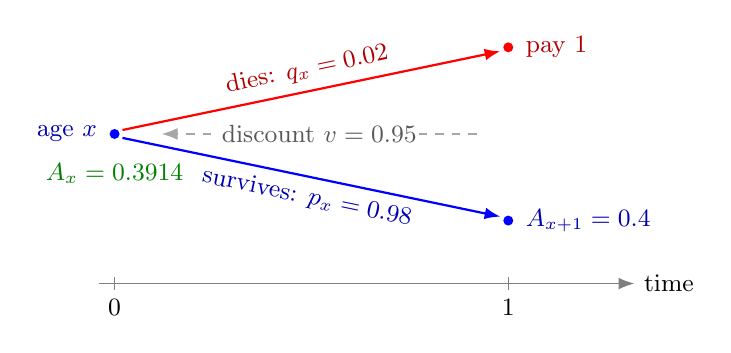
\begin{tikzpicture}[font=\small, >={Latex[length=2mm]}]
  % time axis
  \draw[->, gray] (-0.2,-1.9) -- (6.6,-1.9) node[right, black] {time};
  \draw[gray] (0,-1.82) -- (0,-1.98) node[below, black] {$0$};
  \draw[gray] (5,-1.82) -- (5,-1.98) node[below, black] {$1$};
  % root
  \fill[blue] (0,0) circle (1.8pt);
  \node[blue!70!black, anchor=east] at (-0.1,0) {age $x$};
  \node[green!50!black, anchor=north] at (0,-0.25) {$A_x=0.3914$};
  % branches
  \draw[->, red, thick] (0.1,0.05) -- node[midway, sloped, above, red!70!black] {dies: $q_x=0.02$} (4.9,1.05);
  \draw[->, blue, thick] (0.1,-0.05) -- node[midway, sloped, below, blue!70!black] {survives: $p_x=0.98$} (4.9,-1.05);
  % leaves
  \fill[red] (5,1.1) circle (1.8pt);
  \node[red!70!black, anchor=west] at (5.1,1.1) {pay $1$};
  \fill[blue] (5,-1.1) circle (1.8pt);
  \node[blue!70!black, anchor=west] at (5.1,-1.1) {$A_{x+1}=0.4$};
  % discounting
  \draw[->, gray!70, dashed] (4.6,0) -- (0.6,0);
  \node[gray!70!black, fill=white, inner sep=1pt] at (2.6,0) {discount $v=0.95$};
\end{tikzpicture}
\end{document}
